% ============================================================
% Template LaTeX ABNT NBR 14724/2024 — IFB
% Compatível com pdflatex/xelatex + abntex2 (opcional)
% Gerado via pandoc: pandoc input.md --template=abnt_template.latex -o output.tex
% ============================================================

\documentclass[
  12pt,
  a4paper,
  oneside,
  brazil,
  chapter=TITLE
]{article}

% ── Codificação e Idioma ──────────────────────────────────────────────────────
\usepackage[T1]{fontenc}
\usepackage[utf8]{inputenc}
\usepackage[brazil]{babel}

% ── Fonte Times New Roman (ABNT permite Times New Roman ou Arial) ─────────────
\usepackage{mathptmx}  % Times New Roman para texto e matemática

% ── Geometria da página — margens ABNT anverso ────────────────────────────────
\usepackage[
  a4paper,
  left=3cm,
  top=3cm,
  right=2cm,
  bottom=2cm,
  headheight=14pt,
  headsep=0.5cm
]{geometry}

% ── Espaçamento 1,5 entre linhas (ABNT) ──────────────────────────────────────
\usepackage{setspace}
\onehalfspacing

% ── Recuo do parágrafo: 1,25cm (ABNT) ────────────────────────────────────────
\usepackage{indentfirst}
\setlength{\parindent}{1.25cm}
\setlength{\parskip}{0pt}

% ── Formatação de seções — numeração progressiva NBR 6024 ────────────────────
\usepackage{titlesec}

% Seção primária: MAIÚSCULA, negrito, 12pt, alinhada à esquerda
\titleformat{\section}
  {\normalfont\normalsize\bfseries\MakeUppercase}
  {\thesection\quad}
  {0em}{}

% Seção secundária: caixa baixa, negrito, 12pt
\titleformat{\subsection}
  {\normalfont\normalsize\bfseries}
  {\thesubsection\quad}
  {0em}{}

% Seção terciária: caixa baixa, negrito+itálico, 12pt
\titleformat{\subsubsection}
  {\normalfont\normalsize\bfseries\itshape}
  {\thesubsubsection\quad}
  {0em}{}

% Seção quaternária: caixa baixa, itálico sem negrito, 12pt
\titleformat{\paragraph}[runin]
  {\normalfont\normalsize\itshape}
  {\theparagraph\quad}
  {0em}{}[\hspace{0.5em}]

% Seção quinária: caixa baixa, sem negrito, sem itálico, 12pt
\titleformat{\subparagraph}[runin]
  {\normalfont\normalsize}
  {\thesubparagraph\quad}
  {0em}{}[\hspace{0.5em}]

% Espaçamento das seções — ABNT NBR 14724: separado do texto por linha em branco
% \titlespacing*{cmd}{left}{before-sep}{after-sep}
\titlespacing*{\section}      {0pt}{18pt}{12pt}
\titlespacing*{\subsection}   {0pt}{18pt}{6pt}
\titlespacing*{\subsubsection}{0pt}{12pt}{6pt}
\titlespacing*{\paragraph}    {0pt}{12pt}{0pt}

% Seções primárias iniciam em nova página
\newcommand{\secbreak}{\clearpage}
\let\oldsection\section
\renewcommand{\section}{\secbreak\oldsection}

% ── Numeração de páginas — canto superior direito, 10pt, sem tracas ──────────
\usepackage{fancyhdr}
\pagestyle{fancy}
\fancyhf{}
\fancyhead[R]{\fontsize{10}{12}\selectfont\thepage}
\renewcommand{\headrulewidth}{0pt}
\renewcommand{\footrulewidth}{0pt}

% Primeira página (folha de rosto): sem número visível
\fancypagestyle{plain}{
  \fancyhf{}
  \fancyhead[R]{\fontsize{10}{12}\selectfont\thepage}
  \renewcommand{\headrulewidth}{0pt}
}

% ── Tabelas e Quadros ─────────────────────────────────────────────────────────
\usepackage{longtable}
\usepackage{booktabs}
\usepackage{array}
\usepackage{multirow}
\usepackage{tabularx}

% Estilo de cabeçalho de tabela
\renewcommand{\arraystretch}{1.3}

% Legenda das ilustrações: fonte 10, centralizada (parte superior)
\usepackage{caption}
\DeclareCaptionFormat{abnt}{\fontsize{10}{12}\selectfont#1#2#3}
\captionsetup{
  format=abnt,
  justification=centering,
  singlelinecheck=false,
  labelsep=emdash,      % travessão entre "Quadro 1" e título
  position=above,
  skip=3pt
}

% Comando para fonte abaixo de figuras/quadros (10pt, esquerda)
\newcommand{\fonte}[1]{%
  \begin{flushleft}
    \fontsize{10}{12}\selectfont Fonte: #1
  \end{flushleft}
}

% ── Listas ───────────────────────────────────────────────────────────────────
\usepackage{enumitem}
\setlist{nosep, leftmargin=*}

% ── Sumário e Lista de Quadros (ABNT) ────────────────────────────────────────
\usepackage{tocloft}
\renewcommand{\contentsname}{SUMÁRIO}
% Lista de quadros personalizada
\newlistof{quadros}{loq}{LISTA DE QUADROS}
\setlength{\cftquadrosindent}{0pt}
\setlength{\cftquadrosnumwidth}{0pt}
\makeatletter
\renewcommand{\listofquadros}{%
  \section*{LISTA DE QUADROS}%
  \@starttoc{loq}%
}
\makeatother
% Título do sumário e da lista no mesmo estilo das seções (12pt, negrito)
% Comando: imprime o título em negrito E registra na lista (com número de página)
\newcommand{\quadrotitle}[2]{%
  \vspace{1em}%
  \phantomsection\label{quadro#1}%
  \addcontentsline{loq}{quadros}{Quadro #1 --- #2}%
  \noindent\textbf{Quadro #1 --- #2}\par\vspace{0.3em}%
}
% Linha de fonte do quadro: itálico + espaço após
\newcommand{\quadrofonte}[1]{\par\noindent\textit{Fonte: #1}\vspace{1em}\par}

% ── Hyperlinks ───────────────────────────────────────────────────────────────
\PassOptionsToPackage{hyphens}{url}
\usepackage[hidelinks, colorlinks=false, breaklinks=true]{hyperref}

% ── Citações longas (>3 linhas): 10pt, simples, recuo 4cm ────────────────────
\usepackage{quoting}
\quotingsetup{font=small, indentfirst=false, vskip=\baselineskip}

% ── Suporte a itálico e negrito em nomes científicos / estrangeiros ───────────
\usepackage[normalem]{ulem}

% ── Figuras ──────────────────────────────────────────────────────────────────
\usepackage{graphicx}
\usepackage{float}

% ── Referências ABNT — alinhadas à esquerda, simples, separadas por linha ────
\usepackage[
  alf,
  abnt-emphasize=bf,
  abnt-etal-cite=2,
  abnt-etal-list=0
]{abntex2cite}
% Se abntex2cite não estiver instalado, usar BibLaTeX ou lista manual:
% \usepackage[backend=biber, style=abnt]{biblatex}

% ── Metadados do documento ───────────────────────────────────────────────────
\date{}

% ─────────────────────────────────────────────────────────────────────────────
\begin{document}
% ─────────────────────────────────────────────────────────────────────────────

% ══════════════════════════════════════════════════════════════════════════════
% CAPA — NBR 14724/2024
% ══════════════════════════════════════════════════════════════════════════════
\begin{titlepage}
  \thispagestyle{empty}
  \begin{center}

    % ── Logo IFB + Design de Produto ─────────────────────────────────────────
    
\includegraphics[width=0.4\textwidth]{ifb_vs_dp.png}\\[1.8em]

    % ── Identificação institucional (topo) ────────────────────────────────────
    {\normalsize\bfseries
      Instituto Federal de Educação, Ciência e Tecnologia de Brasília --- IFB\\[0.3em]
      \textit{Campus} Samambaia\\[0.3em]
      Curso Superior de Tecnologia em Design de Produto
    }

    % ── Espaço central ────────────────────────────────────────────────────────
    \vfill

    % ── Título (MAIÚSCULAS, negrito) ──────────────────────────────────────────
    {\large\bfseries
      INDÚSTRIA DE TINTAS E PIGMENTOS NO BRASIL
    }\\[1.2em]

    % ── Subtítulo (caixa baixa) ───────────────────────────────────────────────
    {\normalsize
      Nichos produtivos, matérias-primas e processos de fabricação\\
      na perspectiva da indústria de transformação brasileira.
    }

    \vfill

    % ── Local e ano (rodapé da capa) ──────────────────────────────────────────
    {\normalsize Brasília/DF\\2026}

  \end{center}
\end{titlepage}
\setcounter{page}{2} % contagem inicia na folha de rosto (NBR 14724)

% ══════════════════════════════════════════════════════════════════════════════
% FOLHA DE ROSTO — NBR 14724/2024
% ══════════════════════════════════════════════════════════════════════════════
\begin{titlepage}
  \thispagestyle{empty}
  \begin{center}

    % ── Autor ─────────────────────────────────────────────────────────────────
    {\normalsize\bfseries VICTOR HUGO DA SILVA COSTA}

    \vfill

    % ── Título ────────────────────────────────────────────────────────────────
    {\large\bfseries INDÚSTRIA DE TINTAS E PIGMENTOS NO BRASIL}

    \vfill

    % ── Nota de apresentação (alinhada à direita, ~8cm de largura) ───────────
    \begin{flushright}
      \begin{minipage}{0.5\textwidth}
        \normalsize
        Relatório apresentado ao Curso Superior de Tecnologia em Design de
        Produto do Instituto Federal de Educação, Ciência e Tecnologia de
        Brasília -- IFB -- \textit{Campus} Samambaia, como requisito parcial
        para a aprovação na disciplina de Materiais e Processos de Fabricação~I.

        \vspace{1em}
        Profª.\ Keila Sanches
      \end{minipage}
    \end{flushright}

    \vfill

    % ── Local e ano ───────────────────────────────────────────────────────────
    {\normalsize Brasília/DF -- 2026}

  \end{center}
\end{titlepage}

% ── Demais Elementos Pré-Textuais (adicionar manualmente antes da entrega) ───
% FICHA CATALOGRÁFICA (verso da folha de rosto), FOLHA DE APROVAÇÃO, LISTAS, SUMÁRIO

% ══════════════════════════════════════════════════════════════════════════════
% RESUMO — NBR 6028/2003
% ══════════════════════════════════════════════════════════════════════════════
\clearpage
\thispagestyle{empty}
\begin{center}
  {\normalsize\bfseries RESUMO}
\end{center}

\vspace{1em}
\noindent
O presente trabalho tem como objetivo analisar a indústria brasileira de tintas e pigmentos
na perspectiva da indústria de transformação, identificando os nichos produtivos, as
matérias-primas empregadas e os processos de fabricação característicos de cada segmento.
A metodologia adotada consiste em pesquisa bibliográfica e documental, com base em dados
setoriais da ABRAFATI, do Instituto Brasileiro de Geografia e Estatística (IBGE/PIA-Empresa),
de relatórios de mercado da Grand View Research e da Mordor Intelligence, além de fontes
técnicas especializadas. Os resultados indicam que o Brasil ocupa a 4ª posição no ranking
mundial de produção de tintas, com 2,005 bilhões de litros produzidos em 2025, inserindo-se
em um mercado global avaliado em USD 211,28 bilhões em 2024. O setor estrutura-se como elo
intermediário entre as indústrias de base --- petroquímica, mineração e química fina --- e as
indústrias usuárias, sendo classificado na Divisão 20 da CNAE 2.0. A formulação de tintas
envolve quatro famílias de matérias-primas --- resinas, pigmentos, solventes e aditivos ---
cujas combinações determinam os nichos produtivos identificados: imobiliário, industrial
geral, automotivo, naval, tintas em pó, sistemas de cura UV/EB e tintas especiais e
funcionais. Os processos de fabricação variam conforme o nicho, com destaque para a
dispersão de pigmentos em moinhos de pérolas, a extrusão para tintas em pó e a
fotopolimerização para sistemas de cura por radiação. Conclui-se que o setor apresenta
elevado potencial de diversificação, com nichos estratégicos de alta oportunidade em
anticorrosivos para o segmento offshore, tintas intumescentes, revestimentos para energias
renováveis e sistemas base água, tendência impulsionada por regulamentações ambientais e
pela crescente demanda ESG.

\vspace{1em}
\noindent\textbf{Palavras-chave:} tintas industriais; pigmentos; processos de fabricação; indústria de transformação; nichos produtivos.

% ══════════════════════════════════════════════════════════════════════════════
% ABSTRACT — NBR 6028/2003
% ══════════════════════════════════════════════════════════════════════════════
\clearpage
\thispagestyle{empty}
\begin{center}
  {\normalsize\bfseries ABSTRACT}
\end{center}

\vspace{1em}
\noindent
This paper aims to analyze the Brazilian paint and pigment industry from the perspective of
the manufacturing industry, identifying productive niches, raw materials, and manufacturing
processes characteristic of each segment. The methodology consists of bibliographic and
documentary research, based on sectoral data from ABRAFATI, the Brazilian Institute of
Geography and Statistics (IBGE/PIA-Empresa), market reports from Grand View Research and
Mordor Intelligence, and specialized technical sources. The results indicate that Brazil
ranks 4th in the global paint production ranking, with 2.005 billion liters produced in 2025,
within a global market valued at USD 211.28 billion in 2024. The sector is structured as an
intermediate link between base industries --- petrochemical, mining, and fine chemistry --- and
end-user industries, classified under Division 20 of Brazil's National Classification of
Economic Activities (CNAE 2.0). Paint formulation involves four families of raw materials ---
resins, pigments, solvents, and additives --- whose combinations define the productive niches
identified: residential, general industrial, automotive, naval, powder coatings, UV/EB curing
systems, and specialty and functional paints. Manufacturing processes vary by niche, with
emphasis on pigment dispersion in bead mills, extrusion for powder coatings, and
photopolymerization for radiation-curing systems. It is concluded that the sector presents
high diversification potential, with strategic high-opportunity niches in anticorrosive
coatings for the offshore segment, intumescent paints, renewable energy coatings, and
waterborne systems, a trend driven by environmental regulations and growing ESG demand.

\vspace{1em}
\noindent\textbf{Keywords:} industrial paints; pigments; manufacturing processes; manufacturing industry; productive niches.

% ══════════════════════════════════════════════════════════════════════════════
% LISTA DE QUADROS — NBR 14724/2024
% ══════════════════════════════════════════════════════════════════════════════
\clearpage
\thispagestyle{empty}
\listofquadros

% ══════════════════════════════════════════════════════════════════════════════
% SUMÁRIO — NBR 14724/2024
% ══════════════════════════════════════════════════════════════════════════════
\clearpage
\thispagestyle{empty}
\tableofcontents



\section{INTRODUÇÃO: CONTEXTUALIZAÇÃO DO SETOR NA INDÚSTRIA DE
TRANSFORMAÇÃO
BRASILEIRA}\label{introduuxe7uxe3o-contextualizauxe7uxe3o-do-setor-na-induxfastria-de-transformauxe7uxe3o-brasileira}

A fabricação de tintas, vernizes, esmaltes, lacas e produtos afins está
classificada na \textbf{Divisão 20 da CNAE 2.0} (INSTITUTO BRASILEIRO DE
GEOGRAFIA E ESTATÍSTICA, 2024) (Fabricação de Produtos Químicos),
pertencente à \textbf{indústria de transformação química} --- o segmento
que converte matérias-primas de base petroquímica, mineral e vegetal em
produtos de alto valor agregado.

Trata-se de uma indústria \textbf{genuinamente de transformação}:
insumos sem valor estético ou funcional direto (resinas, pigmentos em
pó, solventes, cargas minerais) são transformados, mediante processos
físico-químicos controlados, em sistemas de proteção e decoração de
superfícies amplamente utilizados por outros elos da cadeia industrial.

\subsection{Posicionamento do Brasil no Cenário Global}\label{posicionamento-do-brasil-no-cenuxe1rio-global}

O Quadro 1 sintetiza os principais indicadores de posicionamento do
Brasil no setor de tintas:

\quadrotitle{1}{Indicadores de posicionamento do Brasil na indústria de tintas (2025)}

{\def\LTcaptype{none} % do not increment counter
\begin{longtable}[]{@{}
  >{\raggedright\arraybackslash}p{(\linewidth - 2\tabcolsep) * \real{0.6471}}
  >{\raggedright\arraybackslash}p{(\linewidth - 2\tabcolsep) * \real{0.3529}}@{}}
\toprule\noalign{}
\begin{minipage}[b]{\linewidth}\raggedright
Indicador
\end{minipage} & \begin{minipage}[b]{\linewidth}\raggedright
Dado
\end{minipage} \\
\midrule\noalign{}
\endhead
\bottomrule\noalign{}
\endlastfoot
Posição no ranking mundial & \textbf{4º maior produtor} (ABRAFATI,
2025) \\
Volume de produção (2025) & \textbf{2,005 bilhões de litros} (ABRAFATI,
2025) \\
Concentração empresarial & Os 10 maiores fabricantes respondem por
\textbf{75\% das vendas} (ABRAFATI, 2025) \\
Empresas associadas (ABRAFATI) & \textbf{70+ fabricantes e
fornecedores} \\
Produção com certificação de qualidade & \textasciitilde{}\textbf{90\%
das tintas imobiliárias} (ABRAFATI, 2025) (\textgreater1 bilhão de
litros/ano) \\
\end{longtable}
}

\quadrofonte{elaborado pelo autor.}

O mercado global de tintas e revestimentos foi avaliado em \textbf{USD
211,28 bilhões em 2024 (GRAND VIEW RESEARCH, 2024)}, com projeção de
atingir \textbf{USD 280,19 bilhões até 2030 (GRAND VIEW RESEARCH, 2024)}
(CAGR de 5,0\%) (GRAND VIEW RESEARCH, 2024). A Ásia-Pacífico detém 35\%
do mercado global (GRAND VIEW RESEARCH, 2024), mas a América Latina ---
com destaque para o Brasil --- é um polo produtor estratégico,
impulsionado pela indústria automotiva, construção civil e agronegócio.

\section{ESTRUTURA DA CADEIA
PRODUTIVA}\label{estrutura-da-cadeia-produtiva}

A indústria de tintas é um \textbf{elo intermediário} na cadeia de
transformação industrial. Sua lógica de funcionamento pode ser descrita
em três camadas (ver Quadro 2):

\quadrotitle{2}{Estrutura da cadeia produtiva da indústria de tintas e pigmentos}

\begin{center}
  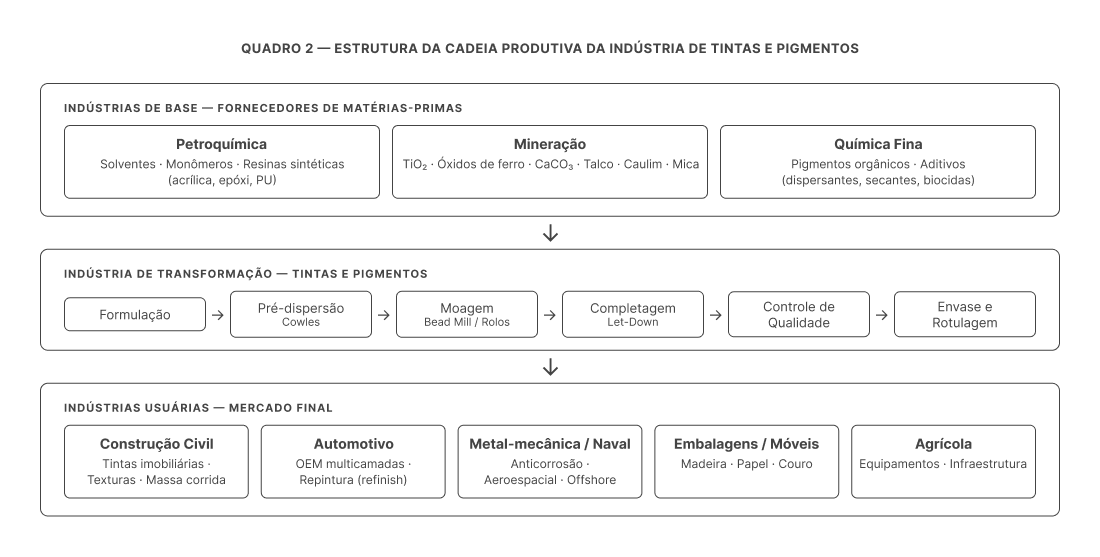
\includegraphics[width=\linewidth]{figuras/quadro2-cadeia-produtiva.png}
\end{center}

\quadrofonte{elaborado pelo autor.}

\section{COMPOSIÇÃO TÉCNICA DAS TINTAS}\label{composiuxe7uxe3o-tuxe9cnica-das-tintas}

Uma tinta é, essencialmente, um \textbf{sistema coloidal} composto por
quatro famílias de matérias-primas, cada qual desempenhando função
específica:

\subsection{Ligantes (Resinas) --- O Formador do
Filme}\label{ligantes-resinas-o-formador-do-filme}

São o componente \textbf{obrigatório e mais nobre} das tintas. Formam a
película protetora após a cura e determinam as propriedades mecânicas,
químicas e de durabilidade (ver Quadro 3).

\quadrotitle{3}{Tipos de resinas (ligantes) utilizados na formulação de tintas: características e aplicações típicas}

{\def\LTcaptype{none} % do not increment counter
\begin{longtable}[]{@{}
  >{\raggedright\arraybackslash}p{(\linewidth - 6\tabcolsep) * \real{0.2500}}
  >{\raggedright\arraybackslash}p{(\linewidth - 6\tabcolsep) * \real{0.2500}}
  >{\raggedright\arraybackslash}p{(\linewidth - 6\tabcolsep) * \real{0.2500}}
  >{\raggedright\arraybackslash}p{(\linewidth - 6\tabcolsep) * \real{0.2500}}@{}}
\toprule\noalign{}
\begin{minipage}[b]{\linewidth}\raggedright
Tipo de Resina
\end{minipage} & \begin{minipage}[b]{\linewidth}\raggedright
Tecnologia
\end{minipage} & \begin{minipage}[b]{\linewidth}\raggedright
Aplicações Típicas
\end{minipage} & \begin{minipage}[b]{\linewidth}\raggedright
Características
\end{minipage} \\
\midrule\noalign{}
\endhead
\bottomrule\noalign{}
\endlastfoot
\textbf{Acrílica} & Base água ou solvente & Imobiliária, repintura
automotiva, industrial & Excelente resistência UV, flexibilidade,
secagem rápida \\
\textbf{Alquídica} & Base solvente & Esmaltes, madeira, metal & Boa
aderência, brilho, cura oxidativa \\
\textbf{Epóxi} & Bicomponente & Pisos, anticorrosivos, naval & Alta
resistência química e mecânica \\
\textbf{Poliuretano (PU)} & Bi ou monocomponente & Automotivo, madeira
nobre, industrial & Resistência à abrasão, flexibilidade, brilho \\
\textbf{Poliéster} & Base solvente & Automotivo, móveis & Alta dureza,
excelente acabamento \\
\textbf{Vinil/PVC} & Base solvente ou água & Naval, piscinas, selantes &
Resistência à umidade e soluções salinas \\
\textbf{Silicone} & Especialidade & Alta temperatura, fachadas &
Resistência extrema a calor e intempéries \\
\textbf{Nitrocelulose} & Base solvente & Madeira, couro & Secagem
ultra-rápida por evaporação \\
\end{longtable}
}

\quadrofonte{elaborado pelo autor.}

\textbf{Tendência dominante:} Resinas acrílicas respondem por
\textasciitilde35,78\% do mercado global (MORDOR INTELLIGENCE, 2026).
Sistemas base água já controlam mais de 50\% do mercado em volume
(MORDOR INTELLIGENCE, 2026), impulsionados por regulamentações
ambientais.

\subsection{Pigmentos --- Cor, Opacidade e
Função}\label{pigmentos-cor-opacidade-e-funuxe7uxe3o}

Os pigmentos são partículas sólidas, finamente divididas, responsáveis
pela \textbf{cor, poder de cobertura, resistência à intempérie e
propriedades funcionais} da tinta. Dividem-se em dois grandes grupos:

\subsubsection{Pigmentos
Inorgânicos}\label{pigmentos-inorguxe2nicos}

Os principais pigmentos inorgânicos utilizados na indústria de tintas,
suas origens minerais e processos de fabricação estão descritos no
Quadro 4:

\quadrotitle{4}{Pigmentos inorgânicos: matéria-prima de origem e processo de fabricação}

{\def\LTcaptype{none} % do not increment counter
\begin{longtable}[]{@{}
  >{\raggedright\arraybackslash}p{(\linewidth - 6\tabcolsep) * \real{0.2500}}
  >{\raggedright\arraybackslash}p{(\linewidth - 6\tabcolsep) * \real{0.2500}}
  >{\raggedright\arraybackslash}p{(\linewidth - 6\tabcolsep) * \real{0.2500}}
  >{\raggedright\arraybackslash}p{(\linewidth - 6\tabcolsep) * \real{0.2500}}@{}}
\toprule\noalign{}
\begin{minipage}[b]{\linewidth}\raggedright
Pigmento
\end{minipage} & \begin{minipage}[b]{\linewidth}\raggedright
Cor
\end{minipage} & \begin{minipage}[b]{\linewidth}\raggedright
Matéria-Prima de Origem
\end{minipage} & \begin{minipage}[b]{\linewidth}\raggedright
Processo de Fabricação
\end{minipage} \\
\midrule\noalign{}
\endhead
\bottomrule\noalign{}
\endlastfoot
\textbf{Dióxido de Titânio (TiO₂)} & Branco & Ilmenita ou rutilo
(minério de titânio) & Processo Sulfato ou Cloreto; calcinação a
800--1000°C \\
\textbf{Óxido de Ferro vermelho (Fe₂O₃)} & Vermelho/marrom & Minério de
ferro (hematita) ou sulfato ferroso & Precipitação, calcinação \\
\textbf{Óxido de Ferro amarelo (FeOOH)} & Amarelo/ocre & Sulfato ferroso
& Precipitação controlada em pH alcalino \\
\textbf{Óxido de Ferro preto (Fe₃O₄)} & Preto & Sulfato ferroso &
Precipitação e redução controlada \\
\textbf{Negro de fumo (Carbon Black)} & Preto intenso & Hidrocarbonetos
(petróleo/gás natural) & Processo furnace (combustão incompleta) \\
\textbf{Cromato de chumbo} & Amarelo/laranja & Cromita, chumbo &
Precipitação química (uso em declínio por toxicidade) \\
\textbf{Azul ultramarino sintético} & Azul & Silicato de alumínio +
enxofre & Calcinação com enxofre a alta temperatura \\
\textbf{Óxido de zinco (ZnO)} & Branco / anticorrosivo & Zinco metálico
ou minério de zinco & Processo direto (oxidação do zinco metálico) \\
\textbf{Litopônio} & Branco & Sulfato de bário + sulfato de zinco &
Reação de precipitação dupla \\
\end{longtable}
}

\quadrofonte{elaborado pelo autor.}

\subsubsection{Pigmentos Orgânicos}\label{pigmentos-orguxe2nicos}

São compostos de síntese orgânica, obtidos majoritariamente da
petroquímica. Oferecem \textbf{alta intensidade de cor e transparência},
sendo amplamente usados em tintas automotivas e industriais (ver Quadro
5).

\quadrotitle{5}{Pigmentos orgânicos: classes, exemplos de compostos e processos de síntese}

{\def\LTcaptype{none} % do not increment counter
\begin{longtable}[]{@{}
  >{\raggedright\arraybackslash}p{(\linewidth - 6\tabcolsep) * \real{0.2500}}
  >{\raggedright\arraybackslash}p{(\linewidth - 6\tabcolsep) * \real{0.2500}}
  >{\raggedright\arraybackslash}p{(\linewidth - 6\tabcolsep) * \real{0.2500}}
  >{\raggedright\arraybackslash}p{(\linewidth - 6\tabcolsep) * \real{0.2500}}@{}}
\toprule\noalign{}
\begin{minipage}[b]{\linewidth}\raggedright
Classe
\end{minipage} & \begin{minipage}[b]{\linewidth}\raggedright
Exemplos
\end{minipage} & \begin{minipage}[b]{\linewidth}\raggedright
Cor
\end{minipage} & \begin{minipage}[b]{\linewidth}\raggedright
Processos de Síntese
\end{minipage} \\
\midrule\noalign{}
\endhead
\bottomrule\noalign{}
\endlastfoot
\textbf{Ftalocianinas} & Azul e verde ftalocianina & Azul, verde &
Síntese por ciclotetramerização do ftalonitrila com metais (Cu, Co) \\
\textbf{Azo-pigmentos} & Vermelho naftol, amarelo hanssa & Amarelo,
laranja, vermelho & Reação de diazotação e acoplamento \\
\textbf{Quinacridona} & PV19, PR122 & Magenta, vermelho & Síntese por
condensação de ácido succínico \\
\textbf{Dioxazina} & Violeta & Violeta & Síntese multiestágio a partir
de cloroanil \\
\textbf{Perileno e Perinona} & Pigmentos de alta performance & Vermelho,
laranja & Condensação de naftaleno diimidas \\
\textbf{Benzimidazolona} & - & Amarelo, marrom, laranja & Síntese
orgânica de precisão \\
\end{longtable}
}

\quadrofonte{elaborado pelo autor.}

\subsubsection{Pigmentos Funcionais
(Especiais)}\label{pigmentos-funcionais-especiais}

Os pigmentos funcionais especiais, suas funções e aplicações industriais
estão sistematizados no Quadro 6:

\quadrotitle{6}{Pigmentos funcionais especiais: tipo, função e aplicações industriais}

{\def\LTcaptype{none} % do not increment counter
\begin{longtable}[]{@{}
  >{\raggedright\arraybackslash}p{(\linewidth - 4\tabcolsep) * \real{0.3333}}
  >{\raggedright\arraybackslash}p{(\linewidth - 4\tabcolsep) * \real{0.3333}}
  >{\raggedright\arraybackslash}p{(\linewidth - 4\tabcolsep) * \real{0.3333}}@{}}
\toprule\noalign{}
\begin{minipage}[b]{\linewidth}\raggedright
Tipo
\end{minipage} & \begin{minipage}[b]{\linewidth}\raggedright
Função
\end{minipage} & \begin{minipage}[b]{\linewidth}\raggedright
Aplicações
\end{minipage} \\
\midrule\noalign{}
\endhead
\bottomrule\noalign{}
\endlastfoot
\textbf{Pigmentos anticorrosivos} (fosfato de zinco, SAPP) & Inibição de
corrosão & Primers industriais, naval \\
\textbf{Pigmentos condutores} (grafite, negro de fumo especial) &
Condutividade elétrica & Revestimentos antiestáticos \\
\textbf{Pigmentos termocromáticos} & Mudança de cor por temperatura &
Indicadores industriais, segurança \\
\textbf{Pigmentos luminescentes} & Reflexão/emissão de luz &
Sinalização, segurança \\
\textbf{Pigmentos perláceos} (mica + TiO₂) & Efeito metálico/perolado &
Automotivo, cosméticos industriais \\
\textbf{Pigmentos antifúngicos} & Biocida integrado & Tintas para
ambientes úmidos \\
\end{longtable}
}

\quadrofonte{elaborado pelo autor.}

\subsection{Solventes e Veículos --- O Meio de
Aplicação}\label{solventes-e-veuxedculos-o-meio-de-aplicauxe7uxe3o}

Responsáveis por ajustar a \textbf{viscosidade e trabalhabilidade}, não
integram o filme final (evaporam após aplicação). Representam um dos
maiores custos e um dos principais focos de redução ambiental (COV ---
Compostos Orgânicos Voláteis) (ver Quadro 7).

\quadrotitle{7}{Solventes e veículos utilizados em tintas: categoria, base química e uso típico}

{\def\LTcaptype{none} % do not increment counter
\begin{longtable}[]{@{}
  >{\raggedright\arraybackslash}p{(\linewidth - 6\tabcolsep) * \real{0.2500}}
  >{\raggedright\arraybackslash}p{(\linewidth - 6\tabcolsep) * \real{0.2500}}
  >{\raggedright\arraybackslash}p{(\linewidth - 6\tabcolsep) * \real{0.2500}}
  >{\raggedright\arraybackslash}p{(\linewidth - 6\tabcolsep) * \real{0.2500}}@{}}
\toprule\noalign{}
\begin{minipage}[b]{\linewidth}\raggedright
Categoria
\end{minipage} & \begin{minipage}[b]{\linewidth}\raggedright
Exemplos
\end{minipage} & \begin{minipage}[b]{\linewidth}\raggedright
Base Química
\end{minipage} & \begin{minipage}[b]{\linewidth}\raggedright
Uso Típico
\end{minipage} \\
\midrule\noalign{}
\endhead
\bottomrule\noalign{}
\endlastfoot
\textbf{Água} & --- & --- & Tintas látex, PVA, acrílicas base água \\
\textbf{Hidrocarbonetos alifáticos} & Varsol, mineral spirit, aguarrás &
Petróleo & Esmaltes alquídicos, imobiliária solvente \\
\textbf{Hidrocarbonetos aromáticos} & Tolueno, xileno & Petroquímica &
Epóxi, poliuretanos, primers \\
\textbf{Álcoois} & n-Butanol, isopropanol & Fermentação/petroquímica &
Poliuretanos, vernizes \\
\textbf{Ésteres} & Acetato de butila, acetato de etila & Petroquímica &
Automotivo, madeira \\
\textbf{Cetonas} & MEK (metil-etil-cetona), MIBK & Petroquímica & Epóxi,
primers de alto desempenho \\
\textbf{Éteres de glicol} & Butilglicol, propilenoglicol & Petroquímica
& Tintas base água (coalescentes) \\
\end{longtable}
}

\quadrofonte{elaborado pelo autor.}

\subsection{Cargas Minerais (Extenders) --- Volume e
Reologia}\label{cargas-minerais-extenders-volume-e-reologia}

Matérias-primas minerais de menor custo que complementam os pigmentos,
ajustando consistência, textura e espessura de película sem contribuir
com opacidade (ver Quadro 8):

\quadrotitle{8}{Cargas minerais (\emph{extenders}): origem mineral e função na formulação de tintas}

{\def\LTcaptype{none} % do not increment counter
\begin{longtable}[]{@{}
  >{\raggedright\arraybackslash}p{(\linewidth - 4\tabcolsep) * \real{0.3333}}
  >{\raggedright\arraybackslash}p{(\linewidth - 4\tabcolsep) * \real{0.3333}}
  >{\raggedright\arraybackslash}p{(\linewidth - 4\tabcolsep) * \real{0.3333}}@{}}
\toprule\noalign{}
\begin{minipage}[b]{\linewidth}\raggedright
Carga
\end{minipage} & \begin{minipage}[b]{\linewidth}\raggedright
Origem Mineral
\end{minipage} & \begin{minipage}[b]{\linewidth}\raggedright
Função Principal
\end{minipage} \\
\midrule\noalign{}
\endhead
\bottomrule\noalign{}
\endlastfoot
\textbf{Carbonato de cálcio (CaCO₃)} & Calcário, mármore & Volume,
redução de custo, textura \\
\textbf{Talco} & Silicato de magnésio & Antisedimentação, matidade \\
\textbf{Caulim} & Argilomineral & Opacidade secundária, reologia \\
\textbf{Baritas (BaSO₄)} & Barita mineral & Densidade,
anti-sedimentação \\
\textbf{Mica} & Silicato laminado & Efeito barreira, impermeabilidade \\
\textbf{Sílica} & Quartzo/areias & Textura, matidade, tixotropia \\
\textbf{Dolomita} & CaMg(CO₃)₂ & Volume, efeito barreira \\
\end{longtable}
}

\quadrofonte{elaborado pelo autor.}

\textbf{O Brasil possui amplas reservas} de carbonato de cálcio, caulim,
talco e barita, conferindo vantagem competitiva à cadeia produtiva
nacional.

\subsection{Aditivos --- Engenharia de
Performance}\label{aditivos-engenharia-de-performance}

Incorporados em pequenas quantidades (0,1--3\%), os aditivos são
responsáveis por \textbf{propriedades críticas de desempenho} e
representam o segmento de maior valor agregado por quilograma (ver
Quadro 9):

\quadrotitle{9}{Classes de aditivos para tintas, funções e exemplos de uso}

{\def\LTcaptype{none} % do not increment counter
\begin{longtable}[]{@{}
  >{\raggedright\arraybackslash}p{(\linewidth - 4\tabcolsep) * \real{0.3333}}
  >{\raggedright\arraybackslash}p{(\linewidth - 4\tabcolsep) * \real{0.3333}}
  >{\raggedright\arraybackslash}p{(\linewidth - 4\tabcolsep) * \real{0.3333}}@{}}
\toprule\noalign{}
\begin{minipage}[b]{\linewidth}\raggedright
Classe de Aditivo
\end{minipage} & \begin{minipage}[b]{\linewidth}\raggedright
Função
\end{minipage} & \begin{minipage}[b]{\linewidth}\raggedright
Exemplos de Uso
\end{minipage} \\
\midrule\noalign{}
\endhead
\bottomrule\noalign{}
\endlastfoot
\textbf{Espessantes/Reológicos} & Controle de viscosidade e fluxo &
Evitar escorrimento em superfícies verticais \\
\textbf{Agentes de dispersão} & Estabilizar pigmentos em suspensão &
Prevenir floculação e sedimentação \\
\textbf{Antiespumantes} & Eliminar bolhas na formulação & Tintas base
água \\
\textbf{Biocidas (\emph{in-can})} & Conservar a tinta na embalagem &
Tintas aquosas (vida útil) \\
\textbf{Biocidas (\emph{dry-film})} & Prevenir fungos/algas na película
seca & Tintas para banheiro, fachada \\
\textbf{Estabilizantes UV} & Proteção à degradação solar & Tintas
externas, automotivas \\
\textbf{Secantes} & Catalisar cura oxidativa & Esmaltes alquídicos \\
\textbf{Coalescentes} & Auxiliar formação do filme acrílico & Tintas
látex em baixas temperaturas \\
\textbf{Plastificantes} & Flexibilizar a película & Tintas elásticas,
impermeabilizantes \\
\textbf{Retardantes de chama} & Reduzir inflamabilidade & Tintas
intumescentes, proteção passiva \\
\end{longtable}
}

\quadrofonte{elaborado pelo autor.}

\section{NICHOS PRODUTIVOS
INDUSTRIAIS}\label{nichos-produtivos-industriais}

\subsection{Tintas imobiliárias
(arquitetural)}\label{tintas-imobiliuxe1rias-arquitetural}

O maior segmento do setor, dominante em volume, com
\textasciitilde{}\textbf{90\% da produção nacional} coberta pelo
Programa Setorial de Qualidade (PSQ/ABRAFATI) (ABRAFATI, 2025).
Subdivisões:

\subsubsection{Tintas Látex / Base
Água}\label{tintas-luxe1tex-base-uxe1gua}

\begin{itemize}
\tightlist
\item
  \textbf{Descrição:} Dispersões aquosas de polímeros acrílicos ou PVA
  (acetato de polivinila)
\item
  \textbf{Matérias-primas:} Resina acrílica em emulsão, TiO₂, CaCO₃,
  coalescentes (éteres de glicol), espessantes celulósicos ou HASE,
  biocidas, antiespumantes
\item
  \textbf{Processo de fabricação:}

  \begin{enumerate}
  \def\labelenumi{\arabic{enumi}.}
  \tightlist
  \item
    Pré-mistura de pigmentos e cargas com água e dispersantes (pasta
    pigmentária)
  \item
    Moagem/dispersão em dissolvedor de alto cisalhamento ou moinho de
    pérolas
  \item
    Adição da emulsão acrílica sob agitação lenta
  \item
    Correção de pH (amônia ou aminas)
  \item
    Adição de aditivos funcionais (biocidas, espessante final,
    coalescente)
  \item
    Ajuste de viscosidade e controle de qualidade (Hegman, viscosidade
    Krebs, pH, cor)
  \item
    Filtração e envase
  \end{enumerate}
\item
  \textbf{Nichos:} Tintas econômicas PVA, tintas standard, tintas
  premium acrílicas, texturas e grafiatos
\end{itemize}

\subsubsection{Esmaltes Sintéticos (Base
Solvente)}\label{esmaltes-sintuxe9ticos-base-solvente}

\begin{itemize}
\tightlist
\item
  \textbf{Matérias-primas:} Resina alquídica (óleo de soja/linhaça +
  anidrido ftálico + glicerina/pentaeritritol), solventes naftalínicos,
  pigmentos, secantes (naftenato de cobalto/manganês/chumbo)
\item
  \textbf{Processo:} Dissolução da resina em solvente → moagem do
  pigmento na solução → adição de secantes → ajuste de viscosidade →
  filtração
\end{itemize}

\subsubsection{Texturas e Revestimentos
Decorativos}\label{texturas-e-revestimentos-decorativos}

\begin{itemize}
\tightlist
\item
  \textbf{Matérias-primas:} Emulsão acrílica, sílica grossa, mármores e
  granitos moídos, cargas grosseiras, pigmentos e aditivos
\item
  \textbf{Processo:} Mistura de alta energia → envase em baldes de 20-25
  kg
\end{itemize}

\subsection{Tintas industriais
gerais}\label{tintas-industriais-gerais}

\subsubsection{Anticorrosivas e
Primers}\label{anticorrosivas-e-primers}

\textbf{Um dos nichos de maior valor agregado}, essencial para
infraestrutura, indústria pesada, petróleo \& gás e construção metálica.

\begin{itemize}
\tightlist
\item
  \textbf{Matérias-primas:}

  \begin{itemize}
  \tightlist
  \item
    Resinas epóxi (bisfenol A + epicloridrina), poliamida ou poliamina
    (endurecedor)
  \item
    Pigmentos anticorrosivos: fosfato de zinco, cromato de estrôncio (em
    declínio), SAPP (fosfato de alumínio modificado), zinc-dust
  \item
    Cargas: baritas, talco, silicatos
  \item
    Solventes: xileno, MEK, butanol
  \end{itemize}
\item
  \textbf{Processo:}

  \begin{enumerate}
  \def\labelenumi{\arabic{enumi}.}
  \tightlist
  \item
    Fabricação da base (componente A): dispersão do pigmento na resina
    epóxi diluída
  \item
    Fabricação do endurecedor (componente B): solução de poliamida/amina
    em solvente
  \item
    Embalagem separada (sistemas 2K)
  \item
    Mistura pelo aplicador em proporção definida
  \end{enumerate}
\item
  \textbf{Subnichos:}

  \begin{itemize}
  \tightlist
  \item
    Primers reativos (\emph{wash primer}, fosfatizantes)
  \item
    Primers epóxi de alto teor de sólidos
  \item
    Primers ricos em zinco (ZRP) --- 80-95\% de zinco em pó na película
    seca
  \item
    Primers alquídicos para metal
  \end{itemize}
\end{itemize}

\subsubsection{Tintas de Piso e Pisos
Industriais}\label{tintas-de-piso-e-pisos-industriais}

\begin{itemize}
\tightlist
\item
  \textbf{Matérias-primas:} Resinas epóxi ou poliuretano, agregados de
  sílica, pigmentos inorgânicos
\item
  \textbf{Características:} Alta resistência ao tráfego, agentes
  químicos e abrasão
\item
  \textbf{Processo:} Similar ao anticorrosivo, com maior teor de sólidos
\end{itemize}

\subsubsection{Tintas Intumescentes (Proteção Passiva ao
Fogo)}\label{tintas-intumescentes-proteuxe7uxe3o-passiva-ao-fogo}

\begin{itemize}
\tightlist
\item
  \textbf{Matérias-primas:} Resina base (acrílica, epóxi ou vinílica),
  pentaeritritol (agente carbonizante), melamina (agente de
  insuflamento), polifosfato de amônio (agente ácido), dióxido de
  titânio
\item
  \textbf{Processo:} Mistura de alta energia; o sistema expande 20-50x
  ao ser exposto ao calor, formando espuma protetora
\item
  \textbf{Aplicações:} Estruturas de aço de edifícios, plataformas
  offshore, galpões industriais
\end{itemize}

\subsection{Tintas automotivas}\label{tintas-automotivas}

Nicho de altíssima tecnologia e qualidade, estruturado em
\textbf{sistemas de pintura multicamadas}:

\textbf{Arquitetura do Sistema Automotivo OEM (Original Equipment
Manufacturer)} (ver Quadro 10):

\quadrotitle{10}{Arquitetura do sistema de pintura automotiva OEM (multicamadas)}

\begin{center}
  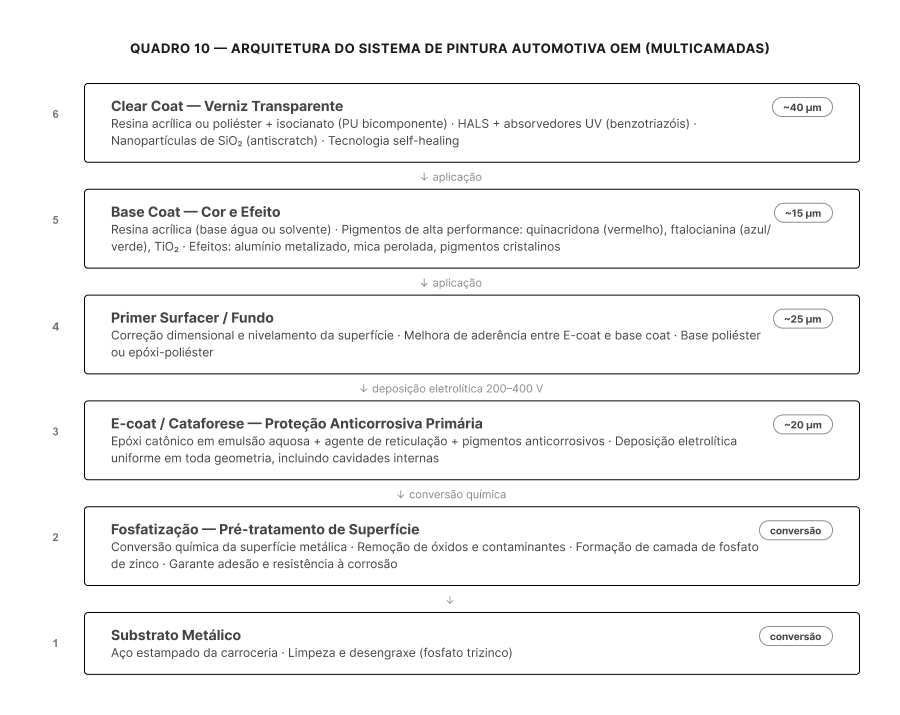
\includegraphics[width=\linewidth]{figuras/quadro10-oem-automotivo.png}
\end{center}

\quadrofonte{elaborado pelo autor.}

\subsubsection{\texorpdfstring{Cataforese
(\emph{E-coat})}{Cataforese (E-coat)}}\label{cataforese-e-coat}

\begin{itemize}
\tightlist
\item
  \textbf{Matérias-primas:} Resina epóxi catônica em emulsão aquosa,
  agente de reticulação, pigmentos anticorrosivos
\item
  \textbf{Processo:} Deposição eletrolítica (200-400V); a peça metálica
  imersa atrai partículas de resina carregadas eletricamente
\item
  \textbf{Resultado:} Película uniforme de \textasciitilde20 µm em toda
  geometria da carroceria, incluindo cavidades
\item
  \textbf{Custo por Risco:} Processo altamente capital-intensivo,
  tecnologia dominada por poucos fornecedores (BASF, PPG, Axalta)
\end{itemize}

\subsubsection{Tintas Base Coat
Automotivas}\label{tintas-base-coat-automotivas}

\begin{itemize}
\tightlist
\item
  \textbf{Matérias-primas:}

  \begin{itemize}
  \tightlist
  \item
    Resina acrílica em emulsão aquosa (base água) ou em solução (base
    solvente)
  \item
    Pigmentos de alta performance: quinacridona (vermelho/magenta),
    ftalocianina (azul/verde), dióxido de titânio, negro de fumo
    especial
  \item
    Pigmentos efeito: alumínio metalizado (efeito metálico), mica
    perolada, pigmentos cristalinos
  \end{itemize}
\item
  \textbf{Tendência:} Base água (\emph{water-borne}) substituiu base
  solvente por regulamentação ambiental (VOC)
\end{itemize}

\subsubsection{Verniz Clear Coat}\label{verniz-clear-coat}

\begin{itemize}
\tightlist
\item
  \textbf{Matérias-primas:} Resina acrílica ou poliéster, isocianato
  (endurecedor para PU), HALS (estabilizantes UV de amina impedida),
  absorvedores UV (benzotriazóis)
\item
  \textbf{Inovação:} Clear coats com proteção antiscratch
  (nanopartículas de SiO₂), ``\emph{self-healing}'' (autorrecuperação
  por calor)
\end{itemize}

\subsubsection{Tintas de Repintura Automotiva
(Refinish)}\label{tintas-de-repintura-automotiva-refinish}

\begin{itemize}
\tightlist
\item
  \textbf{Diferencial:} Cura a temperatura ambiente ou baixa temperatura
  (60-80°C) vs.~140°C no OEM
\item
  \textbf{Matérias-primas:} Sistemas PU de 2 componentes
  (acrílico/poliéster + isocianato alifático), catalisadores, diluentes
  especiais
\item
  \textbf{Mercado no Brasil:} Forte demanda por frota nacional
  envelhecida e acidentes
\end{itemize}

\subsection{Tintas naval e marinha}\label{tintas-naval-e-marinha}

Nicho especializado com demanda crescente da indústria offshore
brasileira (pré-sal), estaleiros e embarcações fluviais/marítimas.

\textbf{Sistemas de Pintura Naval} (ver Quadro 11):

\quadrotitle{11}{Sistemas de pintura naval: camadas, tipos de tinta e funções principais}

{\def\LTcaptype{none} % do not increment counter
\begin{longtable}[]{@{}
  >{\raggedright\arraybackslash}p{(\linewidth - 6\tabcolsep) * \real{0.2500}}
  >{\raggedright\arraybackslash}p{(\linewidth - 6\tabcolsep) * \real{0.2500}}
  >{\raggedright\arraybackslash}p{(\linewidth - 6\tabcolsep) * \real{0.2500}}
  >{\raggedright\arraybackslash}p{(\linewidth - 6\tabcolsep) * \real{0.2500}}@{}}
\toprule\noalign{}
\begin{minipage}[b]{\linewidth}\raggedright
Camada
\end{minipage} & \begin{minipage}[b]{\linewidth}\raggedright
Tipo de Tinta
\end{minipage} & \begin{minipage}[b]{\linewidth}\raggedright
Função
\end{minipage} & \begin{minipage}[b]{\linewidth}\raggedright
Matérias-Primas Principais
\end{minipage} \\
\midrule\noalign{}
\endhead
\bottomrule\noalign{}
\endlastfoot
\textbf{Primer} & Epóxi rico em zinco & Proteção catódica & Zinco em pó,
resina epóxi, endurecedor amina \\
\textbf{Intermediária} & Epóxi \emph{tie-coat} & Reforço anticorrosivo &
Epóxi, pigmentos barreira (mica, óxido de ferro) \\
\textbf{Antincrustante} & Anti-incrustante (\emph{tin-free}) & Prevenir
\emph{biofouling} & Resinas de ablação (acrílico de tributilestanho →
substituído), biocidas (óxido cuproso, Econea®, Sea-Nine) \\
\textbf{Topcoat} & Poliuretano alifático & Proteção UV e estética & PU
base solvente, pigmentos estáveis à intempérie \\
\end{longtable}
}

\quadrofonte{elaborado pelo autor.}

\textbf{O Brasil} possui 7.400 km de costa, a maior frota
\emph{offshore} de petróleo do hemisfério sul (ABRAFATI, 2025) e
extensas hidrovias interiores --- mercado estratégico para tintas
navais.

\subsection{\texorpdfstring{Tintas em pó (\emph{powder
coatings})}{4.5 Tintas em pó (powder coatings)}}\label{tintas-em-puxf3-powder-coatings}

Nicho de crescimento acelerado no Brasil, especialmente na
\textbf{indústria de móveis metálicos, eletrodomésticos, autopeças e
linha branca}.

\begin{itemize}
\tightlist
\item
  \textbf{Descrição:} Sistema 100\% sólido, sem solvente --- eliminação
  total de VOC
\item
  \textbf{Matérias-primas:}

  \begin{itemize}
  \tightlist
  \item
    Resinas sólidas: epóxi, poliéster, híbrido epóxi-poliéster,
    TGIC-poliéster, PU
  \item
    Agentes de cura: diciandiamida (DICY), TGIC, HAA, isocianato
    bloqueado
  \item
    Pigmentos e cargas: TiO₂, pigmentos orgânicos, mica, carbonato
  \item
    Aditivos: niveladores, agentes degassing, catalisadores
  \end{itemize}
\item
  \textbf{Processo de fabricação:}

  \begin{enumerate}
  \def\labelenumi{\arabic{enumi}.}
  \tightlist
  \item
    Pesagem e pré-mistura seca dos componentes
  \item
    Extrusão a 80-120°C (fusão e homogeneização)
  \item
    Resfriamento rápido em rolos frios (chip/flake)
  \item
    Moagem criogênica ou a temperatura ambiente
  \item
    Classificação granulométrica (10-100 µm)
  \item
    Embalagem
  \end{enumerate}
\item
  \textbf{Processo de aplicação:} Pistola eletrostática (corona ou
  tribo) → cura em forno 160-220°C
\end{itemize}

\subsection{Tintas UV/EB (cura por
radiação)}\label{tintas-uveb-cura-por-radiauxe7uxe3o}

\begin{itemize}
\tightlist
\item
  \textbf{Descrição:} Sistemas de cura instantânea por radiação
  ultravioleta ou feixe de elétrons --- sem solvente e alta
  produtividade
\item
  \textbf{Matérias-primas:}

  \begin{itemize}
  \tightlist
  \item
    Oligômeros: acrilatos de epóxi, de uretano (UDA), de poliéster, de
    silicone
  \item
    Monômeros reativos: HDDA, TPGDA, TMPTA (diluentes ativos)
  \item
    Fotoiniciadores: benzofenona, BAPO, TPO (geram radicais livres sob
    UV)
  \end{itemize}
\item
  \textbf{Processo:} Aplicação → passagem sob lâmpada UV (ou LED-UV) →
  polimerização em frações de segundo
\item
  \textbf{Aplicações no Brasil:} Revestimento de madeira e MDF, vernizes
  gráficos, embalagens, eletroeletrônicos, pisos
\end{itemize}

\subsection{Tintas especiais e
funcionais}\label{tintas-especiais-e-funcionais}

\subsubsection{Tintas de Alta
Temperatura}\label{tintas-de-alta-temperatura}

\begin{itemize}
\tightlist
\item
  \textbf{Matérias-primas:} Resinas de silicone puro ou alquil-silicone,
  pigmentos termoestáveis (alumínio, óxido de ferro, espinélios
  metálicos)
\item
  \textbf{Aplicações:} Escapamentos automotivos, fornos industriais,
  chaminés, oleodutos (200--600°C)
\end{itemize}

\subsubsection{Tintas para Embalagens Metálicas (Can
Coatings)}\label{tintas-para-embalagens-metuxe1licas-can-coatings}

\begin{itemize}
\tightlist
\item
  \textbf{Matérias-primas:} Resinas epóxi-fenólicas, acrilatos BPA-free,
  resinas vinil-organossol
\item
  \textbf{Requisito crítico:} Conformidade com legislação de contato
  alimentar (ANVISA/FDA)
\item
  \textbf{Processo:} Aplicação por rolo (\emph{coil coating}) ou spray
  interno nas latas
\end{itemize}

\subsubsection{Tintas Eletroestáticas para Bobinas (Coil
Coatings)}\label{tintas-eletroestuxe1ticas-para-bobinas-coil-coatings}

\begin{itemize}
\tightlist
\item
  \textbf{Matérias-primas:} Resinas poliéster ou PVDF (fluorpolímero),
  pigmentos inorgânicos
\item
  \textbf{Aplicação:} Telhas, painéis de fachada, eletrodomésticos
  (linha branca)
\item
  \textbf{Processo:} Aplicação contínua em linha sobre bobinas de aço
  galvanizado, cura em fornos a \textasciitilde250°C
\end{itemize}

\subsubsection{Tintas Imunomarcantes e de
Segurança}\label{tintas-imunomarcantes-e-de-seguranuxe7a}

\begin{itemize}
\tightlist
\item
  \textbf{Matérias-primas:} Pigmentos fluorescentes, UV-reativos,
  termocrômicos
\item
  \textbf{Aplicações:} Documentos de segurança, embalagens
  anticontrafação, sinalização de emergência
\end{itemize}

\subsubsection{Tintas Anticorrosivas para Petróleo \& Gás}\label{tintas-anticorrosivas-para-petruxf3leo-guxe1s}

\begin{itemize}
\tightlist
\item
  \textbf{Matérias-primas:} Epóxi de alta espessura, poliuretano de alta
  performance, NORSOK/ISO 12944-compliant
\item
  \textbf{Aplicações:} Plataformas offshore Petrobras, dutos, tanques de
  armazenamento
\end{itemize}

\section{PROCESSOS INDUSTRIAIS DE
FABRICAÇÃO}\label{processos-industriais-de-fabricauxe7uxe3o}

\subsection{Fluxograma Geral da Produção de
Tintas}\label{fluxograma-geral-da-produuxe7uxe3o-de-tintas}

O Quadro 12 apresenta o fluxograma geral do processo industrial de
fabricação de tintas:

\quadrotitle{12}{Fluxograma geral do processo industrial de fabricação de tintas}

\begin{center}
  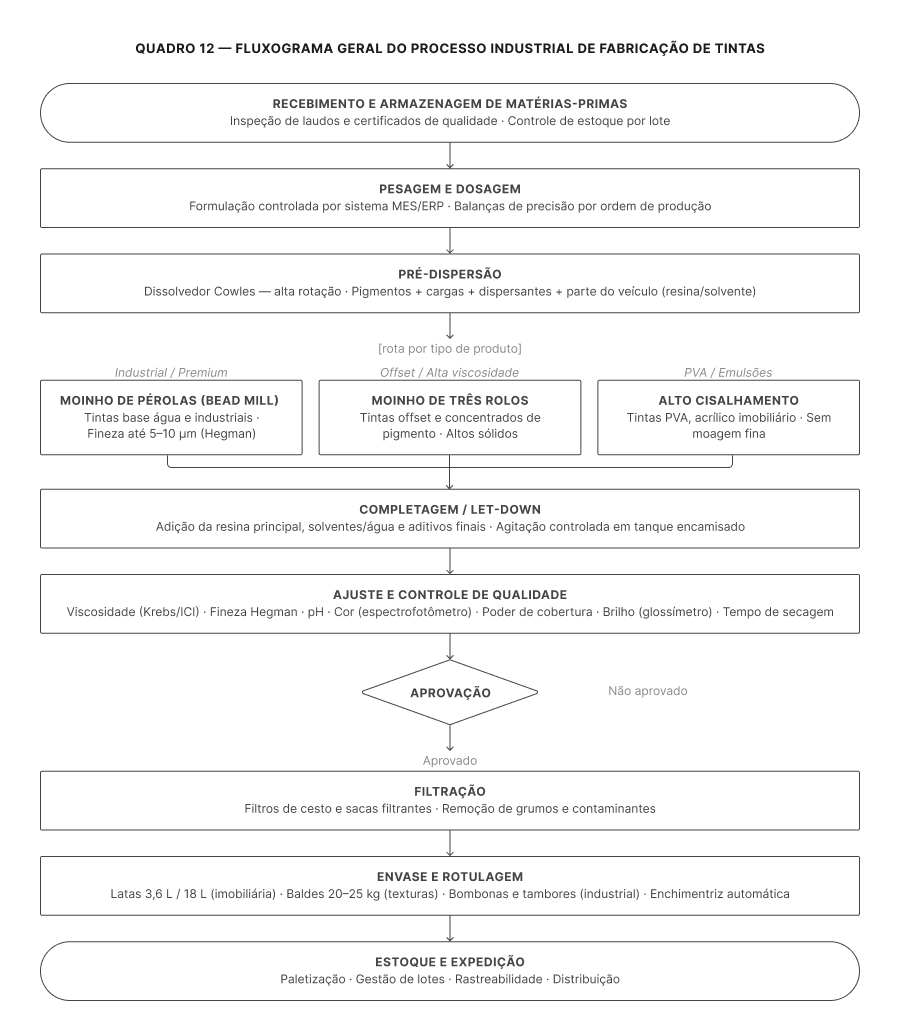
\includegraphics[width=0.85\linewidth]{figuras/quadro12-processo-fabricacao.png}
\end{center}

\quadrofonte{elaborado pelo autor.}

\subsection{Equipamentos Críticos}\label{equipamentos-cruxedticos}

Os equipamentos críticos utilizados na produção industrial de tintas
estão descritos no Quadro 13:

\quadrotitle{13}{Equipamentos críticos na produção de tintas: função e nichos de aplicação}

{\def\LTcaptype{none} % do not increment counter
\begin{longtable}[]{@{}
  >{\raggedright\arraybackslash}p{(\linewidth - 4\tabcolsep) * \real{0.3333}}
  >{\raggedright\arraybackslash}p{(\linewidth - 4\tabcolsep) * \real{0.3333}}
  >{\raggedright\arraybackslash}p{(\linewidth - 4\tabcolsep) * \real{0.3333}}@{}}
\toprule\noalign{}
\begin{minipage}[b]{\linewidth}\raggedright
Equipamento
\end{minipage} & \begin{minipage}[b]{\linewidth}\raggedright
Função
\end{minipage} & \begin{minipage}[b]{\linewidth}\raggedright
Nichos de Aplicação
\end{minipage} \\
\midrule\noalign{}
\endhead
\bottomrule\noalign{}
\endlastfoot
\textbf{Dissolvedor Cowles} & Pré-dispersão de pigmentos & Todas as
linhas \\
\textbf{Moinho de Pérolas (Bead Mill)} & Moagem fina até 5-10 µm &
Industrial, automotivo, tintas premium \\
\textbf{Moinho de Três Rolos} & Moagem de alta viscosidade & Tintas
offset, concentrados de pigmento \\
\textbf{Extrusora de dupla rosca} & Fusão e homogeneização & Tintas em
pó \\
\textbf{Reator de pressão} & Síntese de resinas alquídicas & Fabricantes
verticalizados \\
\textbf{Tanques encamisados} & Mistura com controle de temperatura &
Todas as linhas \\
\textbf{Enchimentriz automática} & Envase em alta velocidade & Tintas
imobiliária e industrial \\
\textbf{Laboratório analítico} & Controle de qualidade & Todas as
plantas \\
\end{longtable}
}

\quadrofonte{elaborado pelo autor.}

\subsection{Processo de Fabricação do Principal Pigmento:
TiO₂}\label{processo-de-fabricauxe7uxe3o-do-principal-pigmento-tioux2082}

O \textbf{dióxido de titânio (TiO₂)} é o pigmento mais importante da
indústria --- presente em \textasciitilde95\% das tintas brancas e como
dispersante de cobertura em tintas coloridas.

\textbf{Processo Sulfato (mais antigo, ainda usado):}

\begin{enumerate}
\def\labelenumi{\arabic{enumi}.}
\tightlist
\item
  Digestão da \textbf{ilmenita (FeTiO₃)} com ácido sulfúrico concentrado
\item
  Dissolução → solução de sulfatos de titânio e ferro
\item
  Hidrólise → precipitação do hidróxido de titânio
\item
  Filtração e lavagem
\item
  Calcinação a 800--900°C → TiO₂ (rutilo ou anatase)
\item
  Tratamento de superfície (SiO₂, Al₂O₃) para estabilização
\end{enumerate}

\textbf{Processo Cloreto (mais moderno e limpo):}

\begin{enumerate}
\def\labelenumi{\arabic{enumi}.}
\tightlist
\item
  Cloração do \textbf{rutilo natural} com cloro gasoso a 900°C → TiCl₄
  (tetracloreto de titânio)
\item
  Purificação do TiCl₄ por destilação fracionada
\item
  Oxidação do TiCl₄ com oxigênio a \textasciitilde1400°C → TiO₂ + Cl₂
  (cloro recuperado)
\item
  Tratamento de superfície inorgânica
\end{enumerate}

\textbf{No Brasil:} A produção de TiO₂ é dependente de importações. O
Brasil possui reservas de ilmenita mas não possui planta industrial de
TiO₂ --- o país importa principalmente de EUA, Alemanha e China (grandes
fornecedores: Chemours, Venator, Kronos, Lomon Billions).

\section{MAPA DE NICHOS × MATÉRIAS-PRIMAS ×
PROCESSOS}\label{mapa-de-nichos-matuxe9rias-primas-processos}

O Quadro 14 apresenta o mapeamento cruzado de nichos industriais com as
respectivas matérias-primas e processos críticos:

\quadrotitle{14}{Mapa de nichos industriais: resina principal, pigmentos, solvente e processo crítico}

{\def\LTcaptype{none} % do not increment counter
\begin{longtable}[]{@{}
  >{\raggedright\arraybackslash}p{(\linewidth - 8\tabcolsep) * \real{0.2000}}
  >{\raggedright\arraybackslash}p{(\linewidth - 8\tabcolsep) * \real{0.2000}}
  >{\raggedright\arraybackslash}p{(\linewidth - 8\tabcolsep) * \real{0.2000}}
  >{\raggedright\arraybackslash}p{(\linewidth - 8\tabcolsep) * \real{0.2000}}
  >{\raggedright\arraybackslash}p{(\linewidth - 8\tabcolsep) * \real{0.2000}}@{}}
\toprule\noalign{}
\begin{minipage}[b]{\linewidth}\raggedright
Nicho Industrial
\end{minipage} & \begin{minipage}[b]{\linewidth}\raggedright
Resina Principal
\end{minipage} & \begin{minipage}[b]{\linewidth}\raggedright
Pigmentos Chave
\end{minipage} & \begin{minipage}[b]{\linewidth}\raggedright
Solvente
\end{minipage} & \begin{minipage}[b]{\linewidth}\raggedright
Processo Crítico
\end{minipage} \\
\midrule\noalign{}
\endhead
\bottomrule\noalign{}
\endlastfoot
Tinta imobiliária látex & Acrílica/PVA em emulsão & TiO₂, CaCO₃, caulim
& Água & Dispersão + emulsificação \\
Esmalte sintético & Alquídica & TiO₂, óxido de ferro & Solvente
naftalínico & Moagem em resina \\
Anticorrosivo primer & Epóxi bicomponente & Fosfato de zinco, TiO₂ &
Xileno/MEK & Dispersão de alta energia \\
Automotivo OEM & Acrílica/poliéster & Pigmentos orgânicos premium & Base
água/solvente & Nanodispersão \\
Repintura automotiva & PU bicomponente & Acrílico/poliéster & Thinner PU
& Mistura 2K \\
Naval \emph{antifouling} & Acrílico de ablação & Óxido cuproso &
Solvente & Dispersão controlada \\
Tinta em pó & Epóxi/poliéster sólido & TiO₂, orgânicos & \textbf{Sem
solvente} & Extrusão + moagem criogênica \\
Coil coating & PVDF/poliéster & Inorgânicos estáveis & Ésteres &
Aplicação de rolo + cura 250°C \\
Cura UV & Acrilatos de uretano & Orgânicos & \textbf{Sem solvente} &
Extrusão + fotoiniciação UV \\
Alta temperatura & Silicone puro & Alumínio, espinélios & Solvente/base
água & Mistura a baixa temperatura \\
Intumescente & Acrílica/epóxi & TiO₂ + sistema intumescente & Base
água/solvente & Mistura controlada de 4 componentes \\
\end{longtable}
}

\quadrofonte{elaborado pelo autor.}

\section{PANORAMA DA INDÚSTRIA DE TRANSFORMAÇÃO NO
BRASIL}\label{panorama-da-induxfastria-de-transformauxe7uxe3o-no-brasil}

\subsection{Estrutura de Mercado}\label{estrutura-de-mercado}

\begin{itemize}
\tightlist
\item
  \textbf{Concentração:} Os \textbf{10 maiores fabricantes} respondem
  por 75\% das vendas (ABRAFATI, 2025) → mercado oligopolizado no topo,
  com centenas de fabricantes médios e pequenos no segmento imobiliário
  regional
\item
  \textbf{Empresas líderes no Brasil:} Suvinil (BASF), Coral
  (AkzoNobel), Sherwin-Williams (com Lazzuril/Colorgin), Renner Tintas,
  Tintas MC, Pintuco, Eucatex Tintas
\item
  \textbf{Modelo de negócio:} As maiores empresas são filiais de
  multinacionais (BASF, AkzoNobel, Sherwin-Williams, PPG, Axalta) que
  dominam os segmentos automotivo e industrial de alta performance; o
  segmento imobiliário tem maior participação de empresas nacionais
\end{itemize}

\subsection{Distribuição Geográfica da
Produção}\label{distribuiuxe7uxe3o-geogruxe1fica-da-produuxe7uxe3o}

A distribuição regional da produção de tintas no Brasil está sintetizada
no Quadro 15:

\quadrotitle{15}{Distribuição geográfica da produção de tintas no Brasil por região}

{\def\LTcaptype{none} % do not increment counter
\begin{longtable}[]{@{}
  >{\raggedright\arraybackslash}p{(\linewidth - 2\tabcolsep) * \real{0.5000}}
  >{\raggedright\arraybackslash}p{(\linewidth - 2\tabcolsep) * \real{0.5000}}@{}}
\toprule\noalign{}
\begin{minipage}[b]{\linewidth}\raggedright
Região
\end{minipage} & \begin{minipage}[b]{\linewidth}\raggedright
Característica
\end{minipage} \\
\midrule\noalign{}
\endhead
\bottomrule\noalign{}
\endlastfoot
\textbf{São Paulo} & Polo concentrador --- maior número de fábricas e a
maioria das multinacionais \\
\textbf{Rio Grande do Sul} & Polo expressivo --- Renner Tintas,
Corepla \\
\textbf{Paraná / Santa Catarina} & Clusters ligados ao setor
moveleiro \\
\textbf{Minas Gerais} & Proximidade com mineração (cargas, pigmentos) \\
\textbf{Nordeste} & Expansão de unidades para atender mercado regional
crescente \\
\end{longtable}
}

\quadrofonte{elaborado pelo autor.}

\subsection{Segmentação por Volume (Estimativa
ABRAFATI)}\label{segmentauxe7uxe3o-por-volume-estimativa-abrafati}

A segmentação do mercado brasileiro de tintas por volume é apresentada
de forma estimada no Quadro 16:

\quadrotitle{16}{Segmentação do mercado brasileiro de tintas por volume --- estimativa}

\begin{center}
  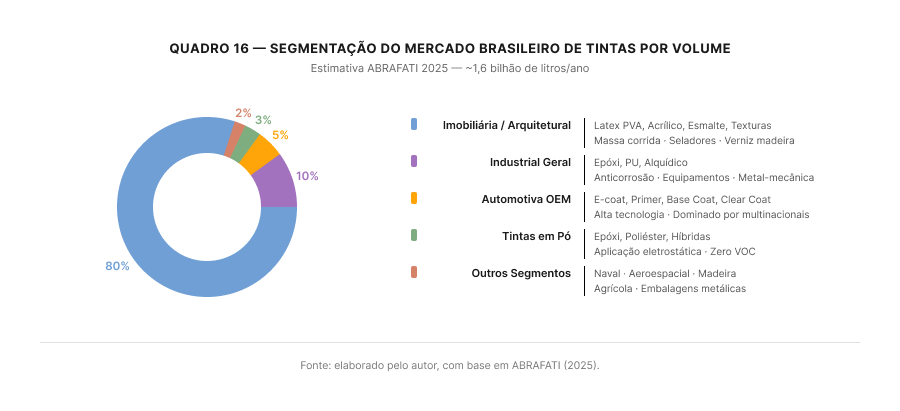
\includegraphics[width=0.9\linewidth]{figuras/quadro16-segmentacao-volume.png}
\end{center}

\quadrofonte{elaborado pelo autor, com base em ABRAFATI (2025).}

\subsection{Principais Elos de Fornecimento de Matérias-Primas no Brasil}\label{principais-elos-de-fornecimento-de-matuxe9rias-primas-no-brasil}

O Quadro 17 lista os principais fornecedores de matérias-primas para a
indústria de tintas no Brasil:

\quadrotitle{17}{Principais fornecedores de matérias-primas para a indústria de tintas no Brasil}

{\def\LTcaptype{none} % do not increment counter
\begin{longtable}[]{@{}
  >{\raggedright\arraybackslash}p{(\linewidth - 2\tabcolsep) * \real{0.5000}}
  >{\raggedright\arraybackslash}p{(\linewidth - 2\tabcolsep) * \real{0.5000}}@{}}
\toprule\noalign{}
\begin{minipage}[b]{\linewidth}\raggedright
Matéria-Prima
\end{minipage} & \begin{minipage}[b]{\linewidth}\raggedright
Principais Fornecedores no Brasil
\end{minipage} \\
\midrule\noalign{}
\endhead
\bottomrule\noalign{}
\endlastfoot
\textbf{Dióxido de Titânio (TiO₂)} & Importado (Chemours, Kronos, Lomon)
--- sem produção nacional \\
\textbf{Resinas acrílicas} & Basf, Allnex, Lubrizol, Acrysol \\
\textbf{Resinas alquídicas} & Resisul, Cargill, Bayer \\
\textbf{Resinas epóxi} & Huntsman, Dow, Hexion \\
\textbf{Óxidos de ferro} & Lanxess, Cathay Industries, produção
nacional \\
\textbf{Carbonato de cálcio} & Omya, Imerys --- vasta produção
nacional \\
\textbf{Caulim} & Imerys Tabatinga (PA), CADAM --- forte base
nacional \\
\textbf{Solventes naftalínicos} & Petrobras Distribuidora, Solvadis \\
\textbf{Aditivos} & BASF, Evonik, BYK-Chemie, Elementis \\
\end{longtable}
}

\quadrofonte{elaborado pelo autor.}

\section{TENDÊNCIAS ESTRATÉGICAS DO
SETOR}\label{tenduxeancias-estratuxe9gicas-do-setor}

\subsection{Transição para Sistemas Base
Água}\label{transiuxe7uxe3o-para-sistemas-base-uxe1gua}

A maior transformação estrutural em curso: sistemas de base aquosa já
dominam \textbf{mais de 50\% do mercado global} e crescem no Brasil por
pressão regulatória (CONAMA, CETESB) e preferência do consumidor. Exige
reformulação de resinas, aditivos e processos.

\subsection{Tintas de Alto Teor de Sólidos (High
Solids)}\label{tintas-de-alto-teor-de-suxf3lidos-high-solids}

Redução de COV mantendo base solvente --- solução para aplicações
industriais que não podem migrar para base água. Requer resinas de menor
massa molecular e processos de aplicação a quente.

\subsection{Nanotecnologia Aplicada}\label{nanotecnologia-aplicada}

\begin{itemize}
\tightlist
\item
  Nanopartículas de TiO₂ fotocatalítico (tintas autolimpantes)
\item
  Nanorevestimentos cerâmicos (automotivo OEM)
\item
  Nanocompósitos de argila (barreira melhorada)
\item
  Nanotubos de carbono (condutividade)
\end{itemize}

\subsection{Matérias-Primas de Base
Renovável}\label{matuxe9rias-primas-de-base-renovuxe1vel}

\begin{itemize}
\tightlist
\item
  Resinas alquídicas a partir de óleos vegetais brasileiros (soja,
  mamona, tungue)
\item
  Solventes derivados de etanol de cana (acetato de etila)
\item
  Pigmentos e corantes de origem biológica
\item
  Óleos essenciais como biocidas
\end{itemize}

\subsection{Economia Circular}\label{economia-circular}

\begin{itemize}
\tightlist
\item
  Programa \textbf{RetornaTinta} (ABRAFATI): coleta e reciclagem de
  tinta residual
\item
  Reaproveitamento de embalagens metálicas
\item
  Formulações com menor geração de resíduos de produção
\end{itemize}

\subsection{Digitalização da
Produção}\label{digitalizauxe7uxe3o-da-produuxe7uxe3o}

\begin{itemize}
\tightlist
\item
  Sistemas de tintometria digital nos pontos de venda (mistura
  personalizada)
\item
  Rastreabilidade de lotes por QR code
\item
  IA para formulação de cores e correspondência de cor (\emph{color
  matching})
\item
  Indústria 4.0 nas plantas: automação de pesagem, dispersão e envase
\end{itemize}

\section{CNAE E CLASSIFICAÇÃO
INDUSTRIAL}\label{cnae-e-classificauxe7uxe3o-industrial}

Para fins de análise da \textbf{Indústria de Transformação} (conforme
IBGE/PIA) (ver Quadro 18):

\quadrotitle{18}{Códigos CNAE 2.0 relacionados à fabricação de tintas, pigmentos e produtos afins}

{\def\LTcaptype{none} % do not increment counter
\begin{longtable}[]{@{}
  >{\raggedright\arraybackslash}p{(\linewidth - 2\tabcolsep) * \real{0.5000}}
  >{\raggedright\arraybackslash}p{(\linewidth - 2\tabcolsep) * \real{0.5000}}@{}}
\toprule\noalign{}
\begin{minipage}[b]{\linewidth}\raggedright
Código CNAE 2.0
\end{minipage} & \begin{minipage}[b]{\linewidth}\raggedright
Descrição
\end{minipage} \\
\midrule\noalign{}
\endhead
\bottomrule\noalign{}
\endlastfoot
\textbf{20.12-6} & Fabricação de intermediários para plastificantes,
resinas e fibras \\
\textbf{20.13-4} & Fabricação de adubos e fertilizantes
organominerais \\
\textbf{20.21-5} & Fabricação de tintas, vernizes, esmaltes e lacas \\
\textbf{20.22-3} & Fabricação de tintas de impressão \\
\textbf{20.23-1} & Fabricação de impermeabilizantes, solventes e
produtos afins \\
\textbf{20.51-7} & Fabricação de produtos de limpeza e polimento \\
\textbf{20.61-4} & Fabricação de adesivos e selantes \\
\textbf{20.62-2} & Fabricação de explosivos e detonantes \\
\textbf{38.39-4} & Recuperação de materiais (inclui reciclagem de
tintas/solventes) \\
\end{longtable}
}

\quadrofonte{elaborado pelo autor.}

\textbf{CNAE principal do setor:} \textbf{20.21-5} --- Fabricação de
tintas, vernizes, esmaltes e lacas

\section{CONSIDERAÇÕES FINAIS: SÍNTESE E OPORTUNIDADES DE
NICHO}\label{considerauxe7uxf5es-finais-suxedntese-e-oportunidades-de-nicho}

\subsection{Nichos de Alta Oportunidade no
Brasil}\label{nichos-de-alta-oportunidade-no-brasil}

O Quadro 19 consolida os nichos de maior oportunidade de mercado para a
indústria de tintas no Brasil, com as respectivas justificativas:

\quadrotitle{19}{Nichos de alta oportunidade para a indústria de tintas no Brasil e justificativas}

{\def\LTcaptype{none} % do not increment counter
\begin{longtable}[]{@{}
  >{\raggedright\arraybackslash}p{(\linewidth - 2\tabcolsep) * \real{0.5000}}
  >{\raggedright\arraybackslash}p{(\linewidth - 2\tabcolsep) * \real{0.5000}}@{}}
\toprule\noalign{}
\begin{minipage}[b]{\linewidth}\raggedright
Nicho
\end{minipage} & \begin{minipage}[b]{\linewidth}\raggedright
Justificativa
\end{minipage} \\
\midrule\noalign{}
\endhead
\bottomrule\noalign{}
\endlastfoot
\textbf{Tintas anticorrosivas offshore} & Expansão do pré-sal, maior
frota offshore do hemisfério sul \\
\textbf{Tintas intumescentes} & Regulamentação crescente (ABNT NBR
14432) e retrofit de edificações \\
\textbf{Tintas em pó (powder)} & Crescimento do setor moveleiro e
eletrodomésticos \\
\textbf{Tintas funcionais agroindustriais} & Silos, tanques de
armazenamento, máquinas agrícolas \\
\textbf{Revestimentos para energias renováveis} & Aerogeradores, painéis
solares (silício + coatings protegidos) \\
\textbf{Tintas de repintura automotiva} & Frota de 120 milhões de
veículos, maior taxa de acidentes do mundo (ABRAFATI, 2025) \\
\textbf{Tintas de base bio (renovável)} & Pressão ESG, oportunidade no
mercado premium \\
\textbf{Coatings para data centers} & Expansão de infraestrutura
digital; tintas antiestáticas e disipadoras \\
\end{longtable}
}

\quadrofonte{elaborado pelo autor.}

\section{REFERÊNCIAS}\label{referuxeancias}

ASSOCIAÇÃO BRASILEIRA DA INDÚSTRIA QUÍMICA. \textbf{ABIQUIM}: Associação
Brasileira da Indústria Química. São Paulo, {[}2026{]}. Disponível em:
\url{https://www.abiquim.org.br}. Acesso em: 9 mar. 2026.

ASSOCIAÇÃO BRASILEIRA DOS FABRICANTES DE TINTAS. \textbf{ABRAFATI}:
anuário do setor de tintas 2025. São Paulo: ABRAFATI, 2025. Disponível
em: \url{https://www.abrafati.com.br}. Acesso em: 9 mar. 2026.

BRITANNICA, The Editors of Encyclopaedia. \textbf{Paint}: chemical
coating. In: BRITANNICA. Chicago: Encyclopædia Britannica, {[}2026{]}.
Disponível em:
\url{https://www.britannica.com/technology/paint-chemical-coating}. Acesso em:
9 mar. 2026.

CHEMEUROPE. \textbf{Paint}. In: CHEMEUROPE ENCYCLOPEDIA. {[}S. l.{]}:
ChemEurope, {[}2026{]}. Disponível em:
\url{https://www.chemeurope.com/en/encyclopedia/Paint.html}. Acesso em: 9 mar.
2026.

GRAND VIEW RESEARCH. \textbf{Paints and coatings market size, share \&
trends analysis report by technology, by application, by region, and
segment forecasts, 2024--2030}. {[}S. l.{]}: Grand View Research, 2024.
Disponível em: \url{https://www.grandviewresearch.com}. Acesso em: 9 mar.
2026.

INSTITUTO BRASILEIRO DE GEOGRAFIA E ESTATÍSTICA. \textbf{Pesquisa
Industrial Anual --- Empresa (PIA-Empresa)}: CNAE 20.21-5. Rio de
Janeiro: IBGE, 2024. Disponível em: \url{https://sidra.ibge.gov.br}. Acesso
em: 9 mar. 2026.

INSTITUTO BRASILEIRO DE GEOGRAFIA E ESTATÍSTICA. \textbf{Classificação
Nacional de Atividades Econômicas --- CNAE 2.0}. Rio de Janeiro: IBGE,
{[}2024{]}. Disponível em: \url{https://concla.ibge.gov.br}. Acesso em: 9 mar.
2026.

MORDOR INTELLIGENCE. \textbf{Paints and coatings market size \& share
analysis --- growth trends \& forecasts (2026--2031)}. {[}S. l.{]}:
Mordor Intelligence, 2026. Disponível em:
\url{https://www.mordorintelligence.com}. Acesso em: 9 mar. 2026.

% ── Elementos Pós-Textuais ───────────────────────────────────────────────────
% REFERÊNCIAS, GLOSSÁRIO, APÊNDICES, ANEXOS

\end{document}
